
%----------------------------------------------------------------------------------------
%	CHAP Seurat
%----------------------------------------------------------------------------------------

\chapterimage{blue-chapter-head_4-reduced.pdf} % Chapter heading image

\chapter{Seurat}\label{chap:Seurat}


\section{The Seurat language}

The Seurat language consists of a series of statements that help with the analysis of
single cell RNA-sequencing data (scRNA-seq data). These statements cover a wide range of
functionality: loading scRNA-seq data, cleaning up the data, adjusting it (by normalization
or scaling), plotting it, computing extra information based on the data (principal components, markers,
etc.), aligning data from multiple samples, performing limma analysis on it and other
functionality.

Seurat statements can be typed in an Analysis script (see Chapter~\ref{chap:Analyses}).
The simplest way to see what Seurat statements are valid at a given line in an
analysis file, is to look at the suggestions offered by the context assistant. Figure~\ref{fig:ContextAssistantBeg}
and Figure~\ref{fig:ContextAssistantMid} show two examples of context assistants.
To activate the context assistant, just press
\keys{\return} in the script to generate an empty line. Placing the cursor on the empty line should
bring up the context assistant; in case you do not see it, press \keys{\space} on the empty line.

\begin{SCfigure}
  \centering
  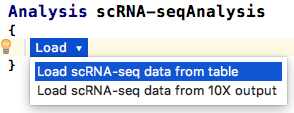
\includegraphics[width=\figWidthTiny]{figures/ContextAssistantBeg.pdf}
\caption[]{}
\label{fig:ContextAssistantBeg.pdf}
\end{SCfigure}

\begin{SCfigure}
  \centering
  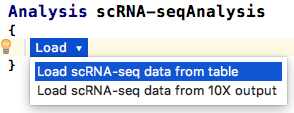
\includegraphics[width=\figWidthTiny]{figures/ContextAssistantBeg.pdf}
\caption[]{}
\label{fig:ContextAssistantBeg.pdf}
\end{SCfigure}

To start writing analyses using Seurat, you need to import devkit 

\noindent The following sections describe the kinds of statements offered by the MetaR
\texttt{org\allowbreak.campagne\allowbreak{}lab\allowbreak.metar\allowbreak.seurat} language.
In these sections, we talk about Seurat objects, but you have to keep in mind that a Seurat
object is a structure that stores scRNA-seq data.

\section{Loading Seurat objects}
\subsection{Load 10X dataset}
\subsection{Load dataset from table}

\section{Cleaning up Seurat objects}
\subsection{Reject gene strategy}
\subsection{Reject cell strategy}
\subsection{Regress out strategy}
\subsection{Accept highly variable genes strategy}
\subsection{Normalization strategy}

\section{Adjusting Seurat objects}
\subsection{Normalize Seurat object}
\subsection{Scale Seurat object}

\section{Plotting Seurat objects}
\subsection{Diagnostic plots}
\subsection{Features plot}
\subsection{Features and total plot}

\section{Adding information to Seurat objects}
\subsection{Add principal component information}
\subsection{Add clusters information}
\subsection{Add markers information}

\section{Aligning Seurat objects}
\subsection{Pre-align Seurat objects}
\subsection{Align Seurat object}

\section{Limma for Seurat objects}
\subsection{Pre-limma Seurat object}
\subsection{Limma voom}

\section{Other Seurat statements}
\subsection{Merge Seurat objects}
\subsection{Delete Seurat object}
